\documentclass[10pt,titlepage]{article}
\usepackage[dvips]{graphics} 
\usepackage{graphicx}
%\usepackage{subfigure}
\usepackage{longtable}
\usepackage{lscape}
\usepackage[pdftex,colorlinks=TRUE]{hyperref}
\setlength{\belowcaptionskip}{0.5cm} % 0.5cm as an example
\raggedbottom
\usepackage[round]{natbib}
\special{papersize=8.5in,11in} \pagestyle{myheadings}
\graphicspath{{figures/}}
\usepackage{fancyhdr}
%\usepackage{fancybox}
%\usepackage{pseudocode}
\pagestyle{fancy}
\lhead{\bf \sc Spherical SOM and Irregular Topology }
\lfoot{Charles R. Schmidt}\rfoot{MS Thesis Proposal}\cfoot{\thepage}
\renewcommand\headrulewidth{1pt}
\renewcommand\footrulewidth{1pt}
\addtolength\oddsidemargin{-2cm}
\addtolength\textwidth{4cm}
\addtolength\headwidth{4cm}
\addtolength\topmargin{-.25in}
\addtolength\textheight{0.25in}
\addtolength\headheight{6pt}
\listfiles
\title{Effects of Irregular Topology in Non-Planar SOM Variants}
\author{\sc{Charles R. Schmidt}\\Regional Analysis Laboratory\\Department of Geography\\San Diego State University}
\date{\today}

\begin{document}
%\maketitle
\break
\begin{center}
{\Large{\bf Effects of Irregular Topology in Non-Planar SOM Variants}}\\*[3mm]
\end{center}
Charles R. Schmidt\\
MS Candidate\\
Department of Geography\\
San Diego State University\\\\
\today\\\break
Committee Members\\
Dr. Sergio Rey, Geography\\
Dr. Andr{\'e} Skupin, Geography\\
Dr. Robert Malouf, Linguistics\\\break
A Thesis Proposal presented to the faculty of San Diego State University.\\
\copyright~2007. Charles R. Schmidt. \\
%% You insert your abstract in the space below.


This document is intended to help students at San Diego State
University to use  \LaTeX\ to produce a Master's Thesis with
high-quality typesetting. Instructions are given for typesetting
complex mathematics and chemical formulas, formatting theorems, using a
variety of table formats, handling figures, and using {\sc Bib}\TeX.  




\\
%\hline
\tableofcontents
\newpage
%\listoffigures
%\newpage
%\listoftables
%\newpage


%
%\documentclass[11pt]{article}
%\setlength{\topmargin}{-.2in}
%\setlength{\oddsidemargin}{-0cm}
%\setlength{\evensidemargin}{-1cm}
%\setlength{\textwidth}{16.3cm}
%\setlength{\textheight}{22.3cm}
%\usepackage{graphicx}
%\usepackage{subfigure}
%\graphicspath{{figures/}}
%\usepackage[round]{natbib}
%\title{Effects of Irregular Topology in Non-Planar SOM Variants}
%\author{\sc{Charles R. Schmidt}\\Regional Analysis Laboratory\\Department of Geography\\San Diego State University}
%\date{\today} %\date{January 29th, 2007}
%\begin{document}
%\maketitle
%\begin{abstract}
%The development of the spherical SOM has been driven by the border effects
%observed in traditional SOM.  Two problems exist with the Spherical SOM. The
%first is the level of control over the network size. The second is the
%topologically induced errors caused by the arrangement of neurons on the sphere.
%Both of these problems stem from the problem of uniformly distributing points on
%a sphere. These problems will be investigated through the introduction of a new
%method for testing topologically induced errors. The method first analyzes  the
%neural network to find topological mis-matches, next we train the network with
%an overwhelming about of synthetic data.  Through a series of simple plots we
%can then compare each neurons internal variance as defined by the variance of
%the observations that best fit that neuron with such metrics as neighborhood
%influence, number of child observations, etc.
%\end{abstract}

\section{Introduction}
The use of a spherical lattice is widely suggested as a solution to the problem
of the boundary effect found in the traditional euclidean Self-Organizing Map
(SOM) \citep{ritter99, boudjemai2003, sangole03, wu2006, Nishio:2006fk}.  The
use of the spherical lattice, however, does not completely overcome this
problem.  With the exception of the five platonic solids, distributing points on
a sphere will always result in irregular network topologies \citep{ritter99,
harris2000}.  The classic method for minimizing this irregularity is to generate
the spherical lattice by tessellating the sides of the icosahedron
\citep{Nishio:2006fk}.  While this method will always result in a highly regular
spherical topology, the main drawback is that the network size, \(N\), grows
exponentially. Other methods for arranging neurons on the sphere allow for
unlimited control over network size, but yield topologies with increased
irregularity \citep{harris2000, wu2005, Nishio:2006fk}.  In order to address the
issue of network size we must first determine the degree to which it is
necessary to minimize the irregularity in these spherical topologies.

\section{Research Objectives}
The objective of this research is to determine the utility of irregular
spherical topologies that offer greater control over network size. Towards that
end, I will develop and test new diagnostics to measure and visualize
topologically induced errors in SOM training.

\begin{itemize}
	\item Develop Diagnostics:
	\begin{enumerate}
		\item Visualize the reverse quantization error by mapping neurons back on to the input data
    		\item Plot: internal variance of each neuron against its first-order neighborhood size
		\item Plot: internal variance of each neuron against the variance in neighborhood size for each topology
	\end{enumerate}
	\item Test Diagnostics with Various Network Topologies
	\begin{enumerate}
    		\item Generate synthetic data
    		\item Train a SOM with comparable parameters for each topology
	\end{enumerate}
\end{itemize}

\section{Background and Lit Review}
The Self-Organizing Map (SOM) is an unsupervised competitive learning process
developed by Teuvo Kohonen as a technique to analyze high dimensional data sets.
The SOM algorithm uses an artificial neural network to organize high dimensional
data onto a low dimensional lattice, or map, of neurons.  Each neuron contains a
reference vector that models the input data.  Before training, these
neuron-vectors are initialized, most commonly to random values.  During the
training process a randomly selected observation (input vector $x$) searches
each neuron (reference vector $m_i$) to find the one to which it is most
similar, referred to as its Best Matching Unit (BMU $c$).  The BMU and its
neighborhood ($N_c$) are then adjusted to better match that observation
\citep{Kohonen2000}.  The training process is repeated a predefined number of
times, or ideally until the map converges.  The traditional SOM is laid out on a
two dimensional plane using either a rectangular or hexagonal topology.
According to \cite{wu2006} the hexagonal structure is more uniform and generally
preferred.

%\subsection{Boundary Effect}
One drawback of building the neural lattice in a discrete euclidean plane is the
boundary of the resulting lattice.  A neuron located on the boundary has fewer
neighbors and thus fewer chances of being updated \citep{wu2006}.  As observed
in Figure \ref{figure1}, neurons in the center of the map tend to better
represent the mean of the input-space.  This is arguably caused by outliers
being pushed to the edges of the map, where they encounter fewer competing
signals.

\begin{figure}
\centering
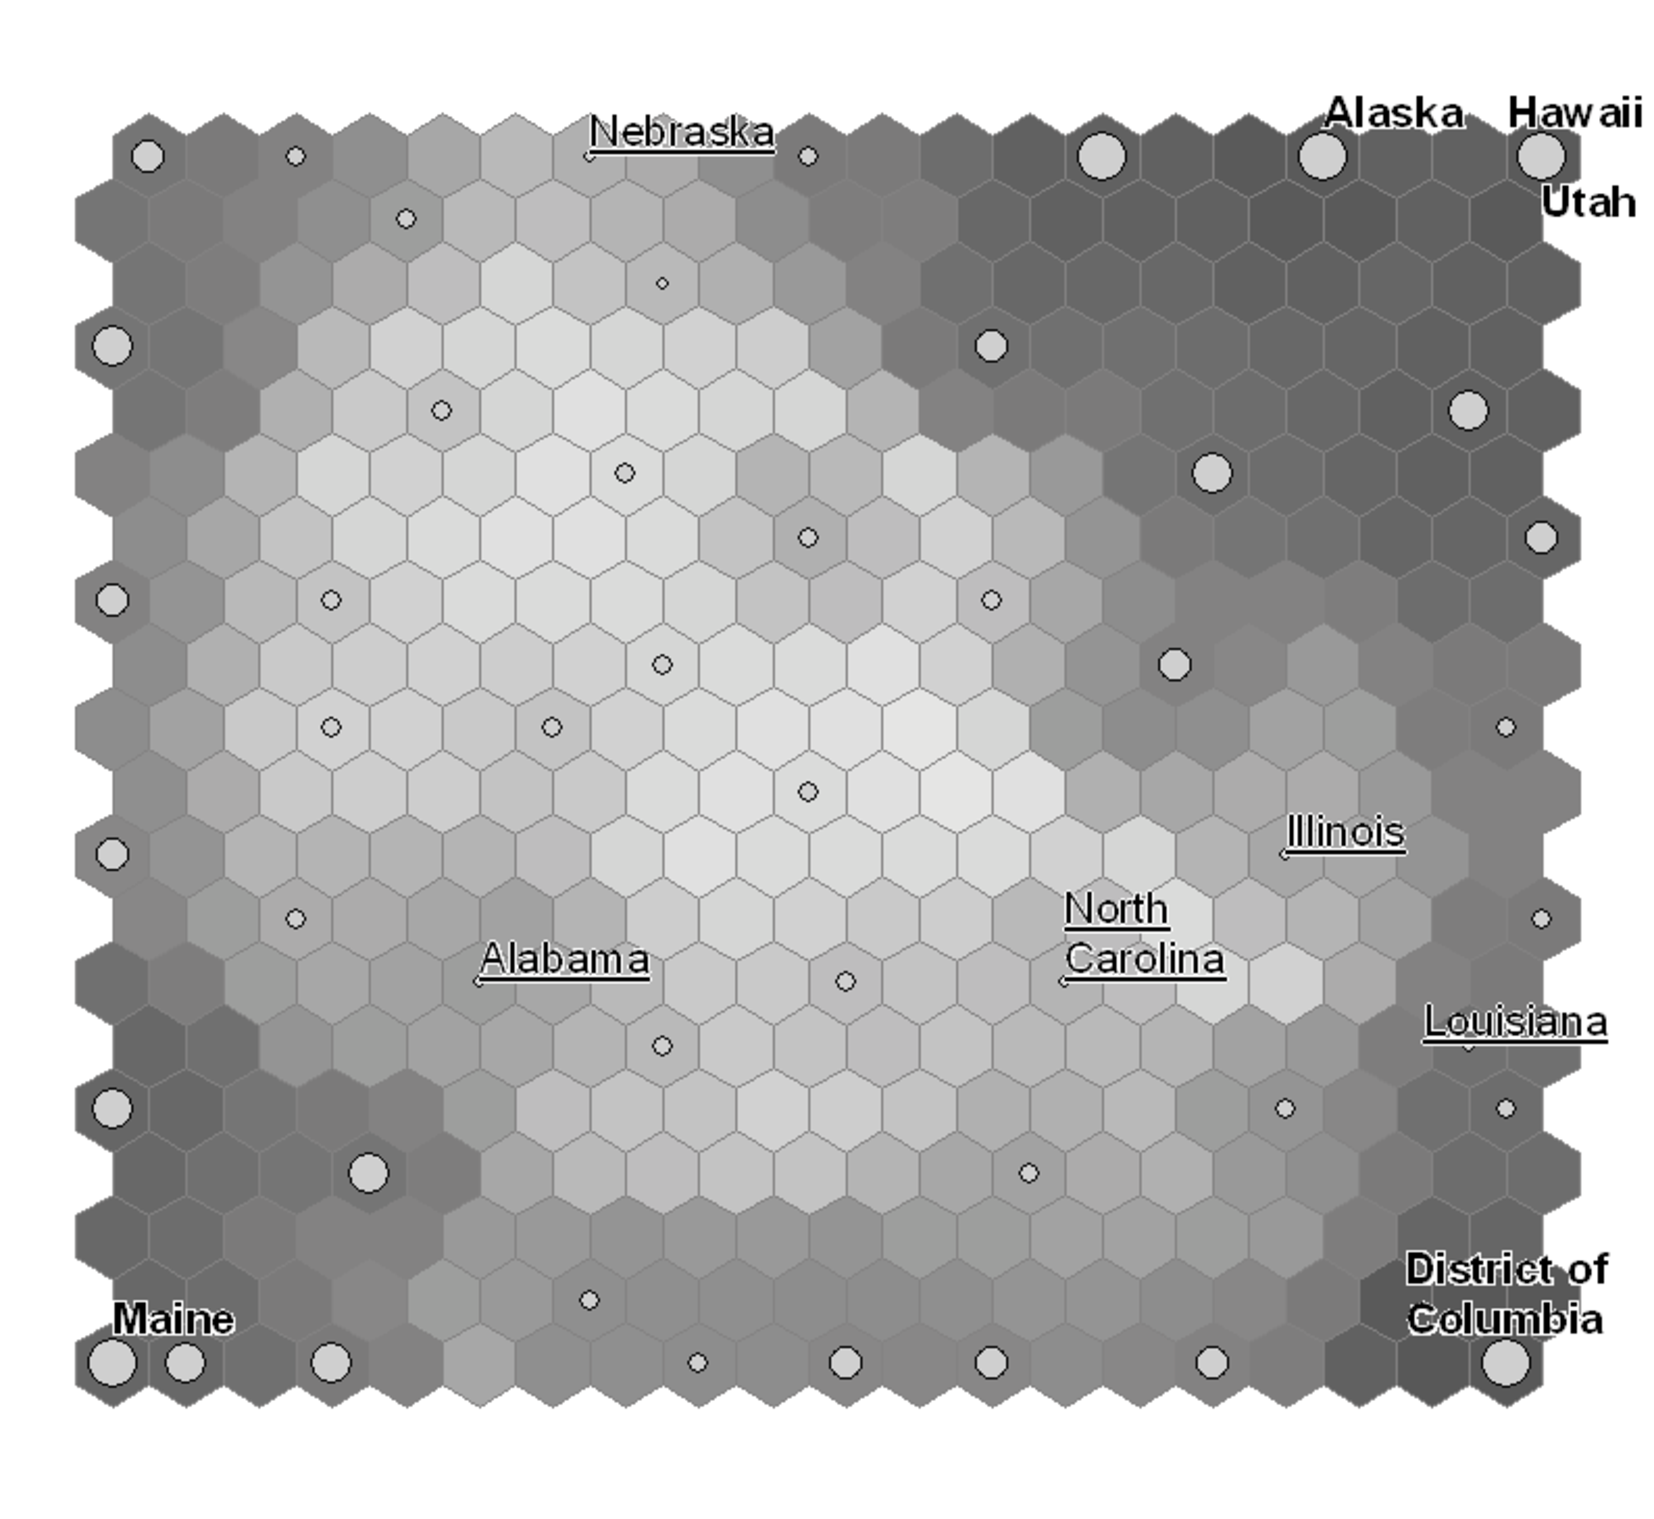
\includegraphics[width=.6\linewidth]{gridedge_grey.pdf}
\caption{Fifty states plus D.C. mapped onto SOM trained with the first
thirty-two census variables.  Darker neurons have a relatively large differences
from the mean of the states, while lighter neurons are relatively closer.
Larger dots represent inputs that were poorly fit to the map, small smaller dots
show inputs that were better bit to the map.}
\label{figure1}
\end{figure}


\subsection{Spherical SOM}
One way to eliminate the boundary effect is to wrap the lattice around a three
dimensional object such as a sphere or torus, thereby removing the edge
entirely. The toroidal SOM was introduced by \cite{li1993}, however the torus is
not hugely effective for visualization, as maps generated from a torus are not
very intuitive \citep{ito2000,wu2006}.  \cite{ritter99} describes the torus as
being topologically flat and suggests that a curved topology, such as that of a
sphere, may better reflect directional data.  A sphere also results in a more
intuitive map, since we are accustomed to looking at maps based on a sphere.

\cite{ritter99} first introduced the spherical SOM and several enhancements have
since been suggested \citep{boudjemai2003,sangole03,Nishio:2006fk,wu2006}.  A
good comparison of these enhancements can be found in \cite{wu2006}.  All of
these methods derive their spherical structure through the tessellation of a
polyhedron as originally proposed by \cite{ritter99}.  \cite{wu2006} point
out the importance of a uniform distribution on the sphere and that it is
preferable for all neurons to have an equal number of neighbors and to be
equally spaced.  They find generally that the tessellation method best satisfies
these conditions and specifically that the icosahedron is the best starting
point \citep{wu2005}. Tessellation of the icosahedron results in a network of
neurons, each of which have exactly six neighbors, save the original twelve
which each have five.  This is very close to the ideal structure in which every
neuron would have exactly six neighbors.  This structure has very low variances
in both neuron spacing and neighborhood size.


\subsection{Network Size}
\begin{figure}
\centering
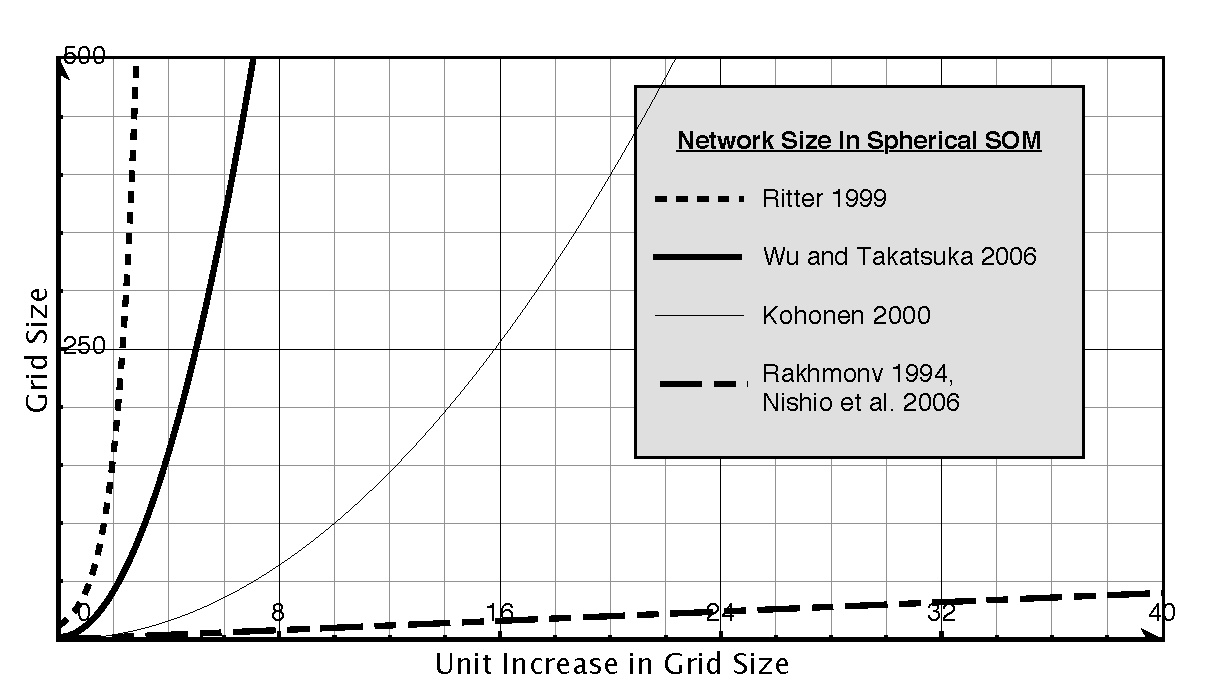
\includegraphics[width=\linewidth]{networkSize.pdf}
\caption{This figure demonstrates the achievable network size using various
spherical topologies.}
\label{fig:nSize}
\end{figure}
The literature offers little theoretical guidance on network size
\citep{cho1996}.  \cite{toolbox} suggests simply using a network size of
\(5*\sqrt {n}\), where \(n\) is the number of observations. Given this lack of
theoretical development, researchers should cautious when using methods that
limit the control of network size.  As shown in Figure \ref{fig:nSize},
methods for arranging an arbitrary number of points on a sphere provide a much
higher degree of flexibility when choosing a network size.

The cost of relying on \citeauthor{ritter99}'s tessellation method is decreased
control over network size. \citeauthor{ritter99}'s tessellation methods results
in a network size that grows at a rate of \(N=2+10*4^f\), where $f$ is the
frequency of tessellation. \cite{wu2006} offer a slight improvement. Rather than
recursively subdividing the faces, they redivide the original icosahedron with
each step resulting in \(N=2+10*f^2\).  In practice 2D Euclidean SOMs also offer
limited control over network size, because it is undesirable to have one dimension
dramatically larger than the other.  \cite{Nishio:2006fk} try to address the
issue of network size granularity by departing from the tessellation method and
suggesting the use of a partitioned helix to uniformly distribute any number of
neurons on a sphere.  A similar method proposed by \cite{Rakhmanov94} was
dismissed by \cite{wu2005} for failing to satisfy the uniformity conditions
described above.

\subsection{Uniformity}
\citeauthor{wu2006} state that ``[f]or SOM, it is desirable to have all neurons
receive equal geometrical treatment'' \cite[pp. 900]{wu2006}.  To satisfy this
constraint two conditions must be met.  Firstly, each neuron should occupy the
same amount of space on the given surface.  Secondly, each neuron should be
bordered by the same number of surrounding neurons, and we should maximize that
number.  The first condition is hugely important for visualization, but
irrelevant for training.  During the training of the SOM only the topology of
the neurons is considered.

Based solely on measures of neuron spacing \cite{wu2005} dismissed a method
proposed by \cite{Rakhmanov94} for distributing points on a sphere.  Similarly
\cite{Nishio:2006fk} use these variance measures to support their helix
algorithm for distributing points on a sphere.  Table \ref{table1} shows that
these metrics can be misleading and may not be comparable across topologies.
The traditional rectangular and hexagonal topologies have no variance in neuron
spacing and the generally preferred hexagonal structure displays greater
variance in neighborhood size than the rectangular structure.  The torus by
comparison would have variance in neuron spacing, yet no variance in
neighborhood size.  The distance between two neurons is only considered during
the formation of the neuronal network.  At this stage the spacing is significant
as it plays a part in determining neuron adjacency. However, using this measure
to evaluate potential topologies for use in SOM may be misleading.

\begin{table}[htbp]
\caption{Variances in Topologies}
\begin{center}
\begin{tabular}{|c|c|c|c|}
\hline
Topology&Grid Size&Neuron Spacing&Variance in Neighborhood Size\\
\hline
Rectangular&9x18&1&0.2716\\
Hexagonal&9x18&1&1.2138\\
Tessellation&162&0.25319 - 0.31287& 0.0686\\
Rakhmanov&162&0.15779 - 0.30069& 0.2908\\
\hline
\end{tabular}
\end{center}
\label{table1}
\end{table}

Methods, for distributing points on the sphere, which allow for fine grained
control over network size produce slightly more irregular topologies.  However,
no discussion of these irregularities or their effects on SOM training has
occurred in the literature. Given that limited theoretical guidance is available
for choosing network size the desire for finer control over the network size,
should not be overlooked. In particular for a larger SOM the ideal network size
may not be achievable via tessellation of the icosahedron.

\section{Data and Methodology}
This section is composed of two parts.  The first of which describes each of
the methods developed for testing network topologies.  The second describes an
empirical study that will implement these methods as well as evaluate their
utility. 

\subsection{Diagnostics}
\subsubsection{Visualize reverse mapping}
The quantization error (QError) of a SOM is a simple way to measure how well 
data matches a trained SOM \citep{Kohonen2000}. The QError is measured by averaging
the euclidean distance between each observation and its best match.  The QError can
be decomposed to show how well each observation fits the SOM.  For the first
diagnostic tool I will find the euclidean distance between each neuron and its
best matching observation.  The result will be a map that shows how well the
neurons fit the data. This can be extended to produce a map that shows the
distances of neurons to the mean (or median) of the input data.

\subsubsection{Plot the internal variance of each neuron against its first-order neighborhood size}
In traditional SOMs, outlying observations are pushed to the edge of the map where
they encounter fewer competing signals. A prime example of this is the
``Utah-Hawaii'' case shown in figure \ref{figure1}.  Relying only on the SOM one
would be left to believe that the two states are similar. Upon closer inspection we see
that the QError from Utah to the neuron is $1.509$, the QError from Hawaii to
the neuron in $1.505$, but the QError from Utah to Hawaii is $3.014$. In this
case only Utah and Hawaii were mapped to that neuron.  In a case where multiple
observations land on the same neuron it is possible to measure average pairwise
QErrors between those observations.  This gives us a notion of internal variance for
each neuron. It would be expected that in traditional SOM neurons closer to the
edge will have higher internal variances. This can be extended to spherical SOM
by comparing the degree of each neuron ($deg(m_i)$ or the number of adjacent
neurons) to its internal variance.

\subsubsection{Plot the internal variance of each neuron against the variance in neighborhood size for each topology}
The degree of each neuron can easily be calculated by taking the column sums of
the first-order adjacency matrix ($A$).  A completely regular network
topology (i.e. the torus) will have no variance in these column sums.  For
irregular networks the variance in these column sums give us a measure of
irregularity.  For each topology type we can plot the internal
variances as described above versus the neighborhood size variance.  We should see
what resembles multiple box plots with higher means as the regularity decreases. 
%It may also be useful to visualize these variances as a map.  This will show us where topologically induced errors are occurring.

\subsection{Empirical Analysis}
\begin{itemize}
\item In order to test the methods described above I will generate synthetic data with
known properties.
\item I will train a SOM for each of several topologies in order to apply the
diagnostics.
\item Knowing the properties of the training data allow us to systematically
compare the diagnostics under several different topologies.
\item To ensure that we can calculate an internal variance for
each neuron I will generate overwhelming amounts of data, increasing the
probability that each neuron will be occupied by more than one observation.
\end{itemize}

%\subsubsection{Synthetic Data} I will take advantage of weights matrices to generate synthetic training data with known properties.  This data will be used to train the various SOMs in order to facilitate comparison.

%\subsubsection{Train SOM}

%It is useful to represent our neural lattice as a graph, G.
%We know that any arrangement of neurons onto the surface of a sphere will as such the network can be effectively treated as a graph.  Doing so enables us to use the properties of the graph and the principles of graph theory to help us understand the relationship between neurons during training.

%the variance in neuron spacing should be minimized.    The first condition ensures that each neuron will occupy is only of concern when visualizing the SOM.

%The get at the second condition we must first define the degree of a neuron, deg(n) to be number of its direct neighbors.  Whit that in mind the second condition is that the variance in the degree of the neurons must also be minimized.

%This statement may be somewhat misleading to those investigating alternative 

%For the purpose of SOM visualization it is important for each neuron to receive equal geometrical treatment.

%It is useful to represent the neural network as a graph, G, in order use the...
%In order to examine the irregularities in the neural network it is useful ....

%The basic problem of the "boundary effect" is that neurons on the edge have fewer neighbors. Yet there are only five possible arrangements of points on a sphere such that all points have the same number of neighbors.  Any spherical lattice consisting of more then twenty (dodecahedron) neurons will contain topological irregularities.  This is to say that not all neurons will have the same number of neighbors.  The importance of these irregularities and the magnitude of their effects on SOM training is not known.  This goal of this research is to determine whether more flexible network structures may be used in spherical in SOM without introducing significant errors. To accomplish this goal, basic methods in network analysis with be combined with the result from several empirical training runs each utilized different topology.  

\bibliographystyle{apalike}
\bibliography{som}
\end{document}
